\subsection{Starbucks}
\subsubsection{Topologia estimada de red}
\begin{figure}[h!]
  \centering	
	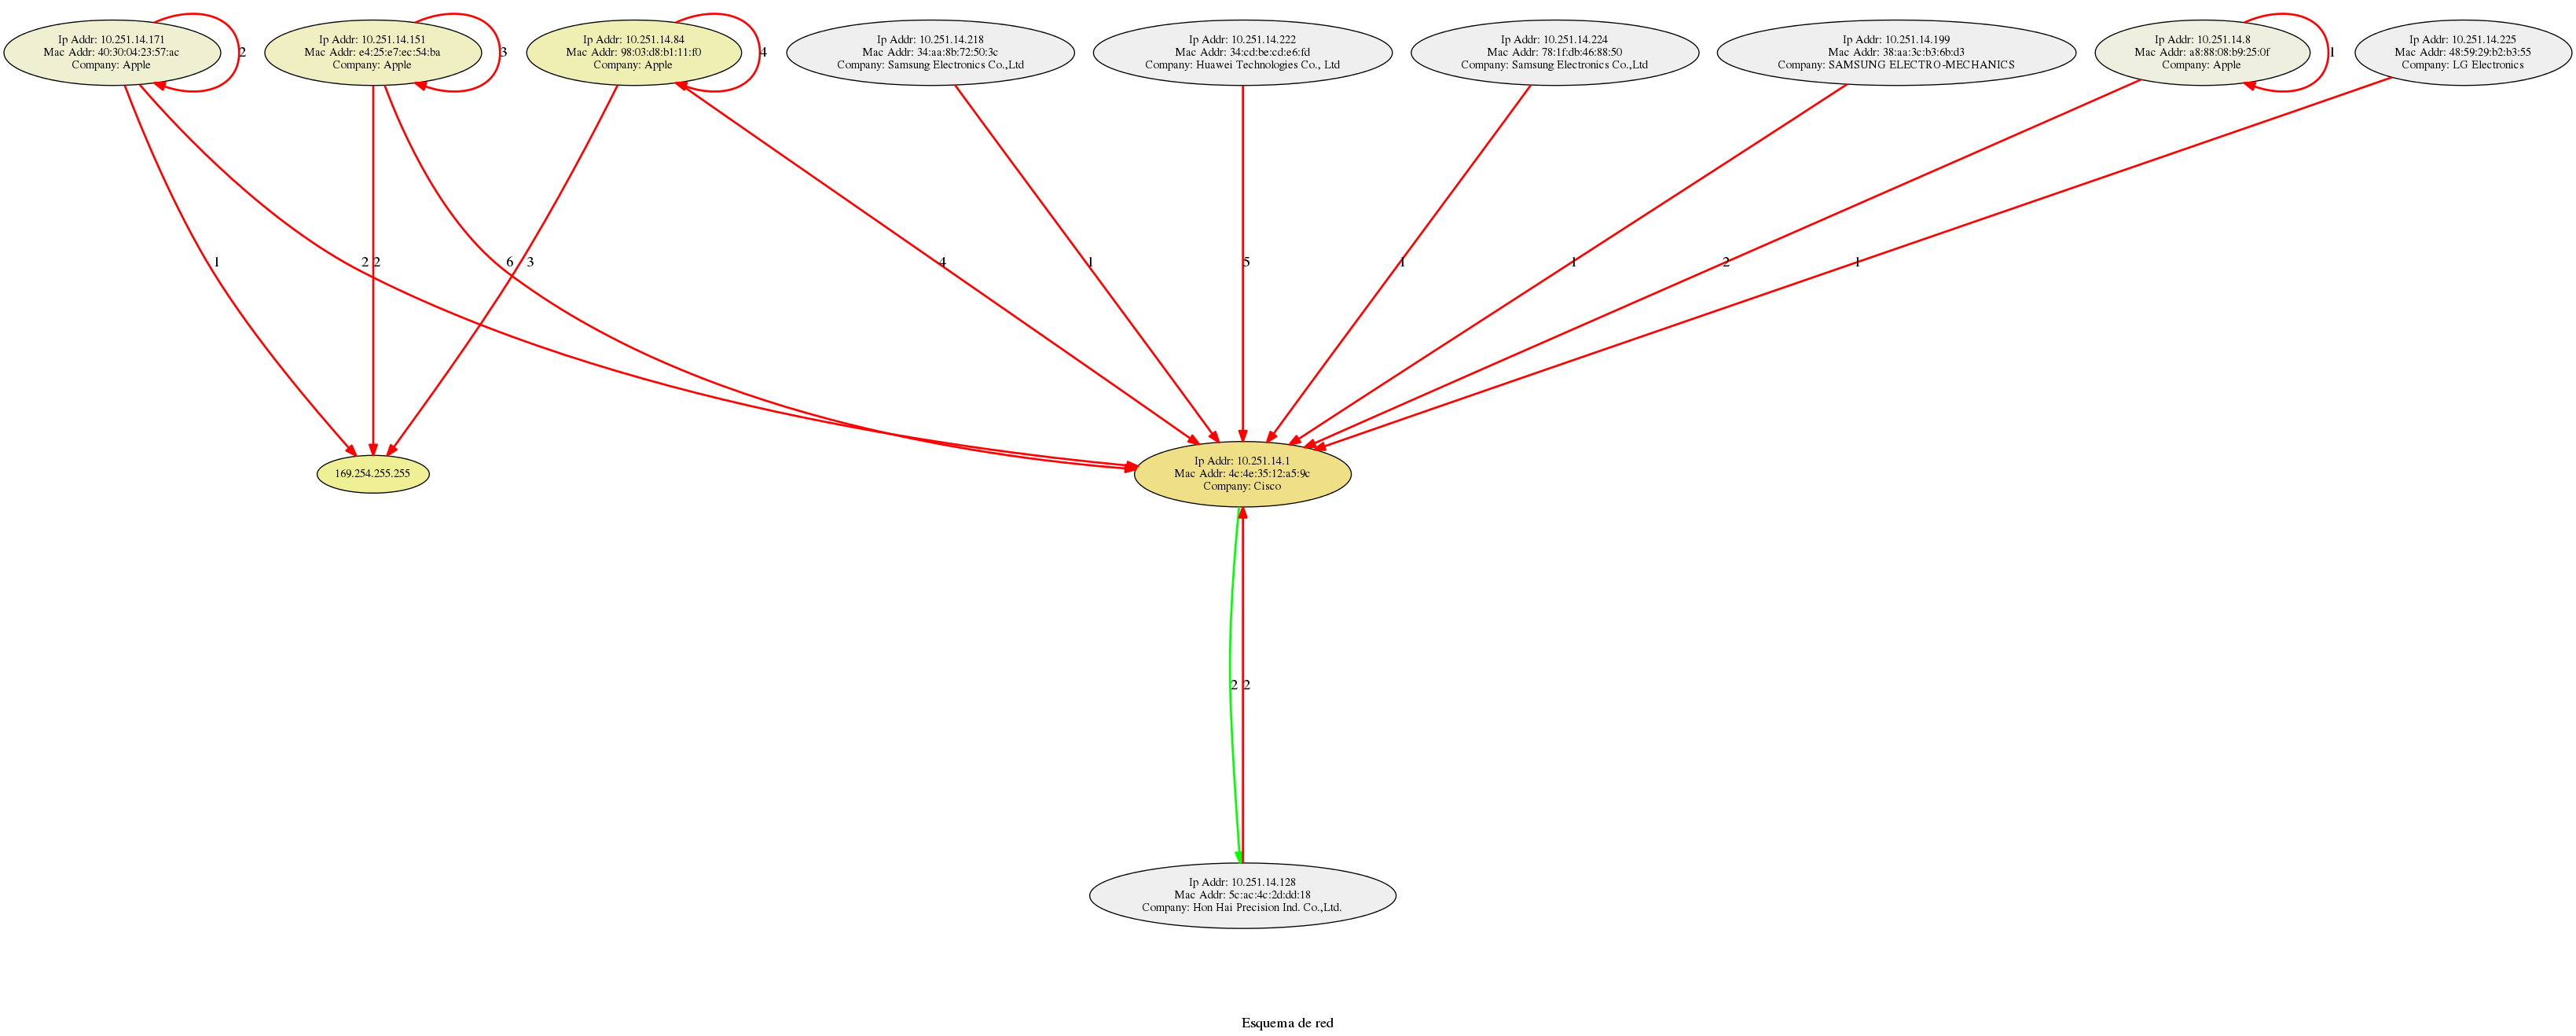
\includegraphics[scale=0.15]{../experimentacion-svilerino/starbucks/graph-starbucks-3.png}
  \caption{(grafo con experimento mas pequeño, el grafo completo puede encontrarse en la carpeta de experimentacion)}
\end{figure}

\subsubsection{Probabilidades y entropia de fuente origen}
\begin{figure}[h!]
  \centering
	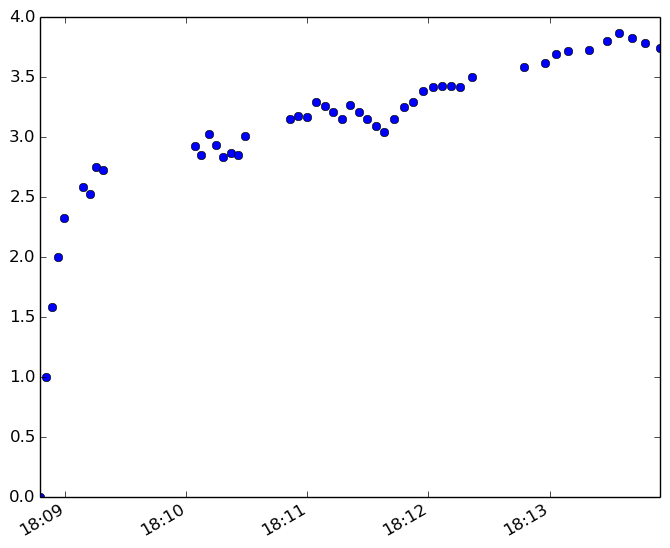
\includegraphics[scale=0.66]{../experimentacion-svilerino/starbucks/full-experiment-1/entropy_src.png}
  \caption{Entropia de la fuente origen.}
\end{figure}

\begin{figure}[h!]
  \centering
	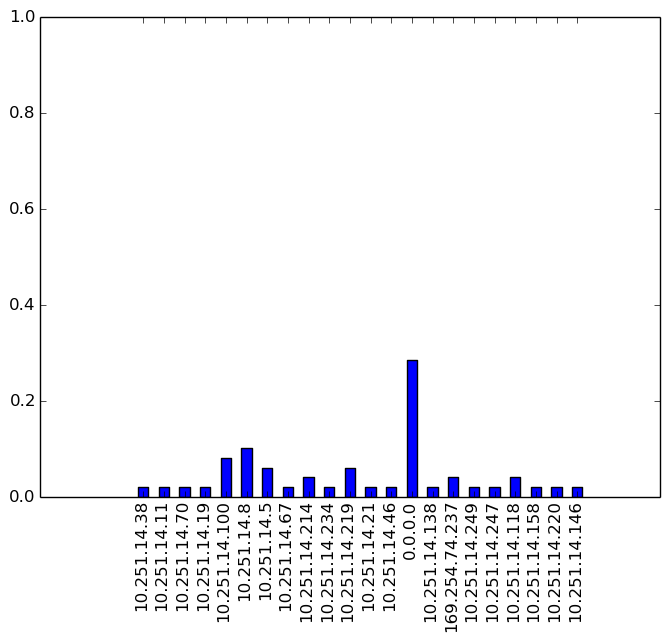
\includegraphics[scale=0.66]{../experimentacion-svilerino/starbucks/full-experiment-1/histogram_src_probabilities.png}
  \caption{Probabilidades asociadas a las IP de la fuente origen.}
\end{figure}

%---------------------------------------------------------------------------------------------------------------

\subsubsection{Probabilidades y entropia de fuente destino}
\begin{figure}[h!]
  \centering
	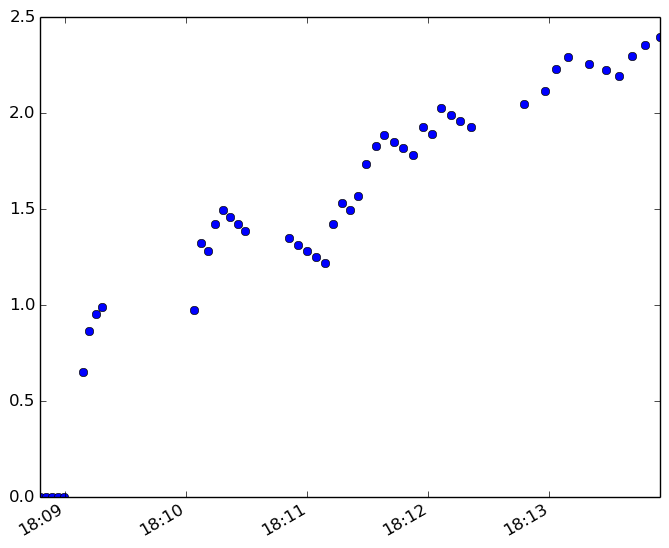
\includegraphics[scale=0.66]{../experimentacion-svilerino/starbucks/full-experiment-1/entropy_dst.png}
  \caption{Entropia de la fuente destino.}
\end{figure}

\begin{figure}[h!]
  \centering
	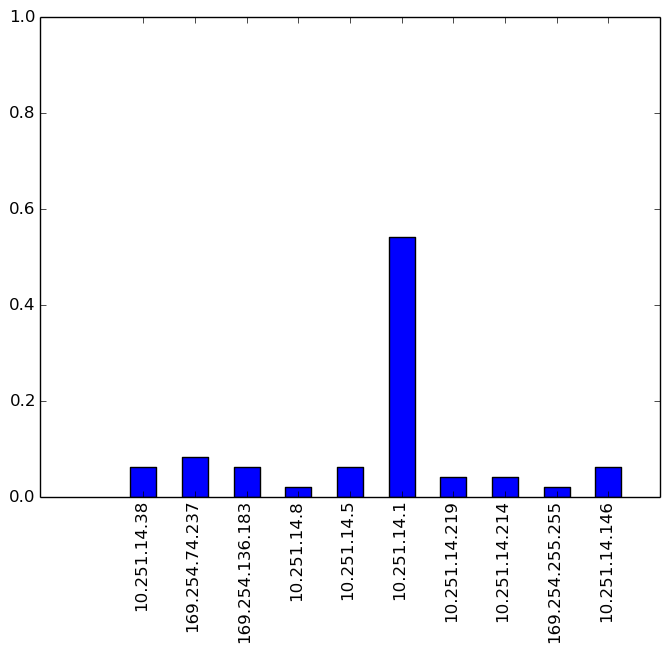
\includegraphics[scale=0.66]{../experimentacion-svilerino/starbucks/full-experiment-1/histogram_dst_probabilities.png}
  \caption{Probabilidades asociadas a las IP de la fuente destino.}
\end{figure}

\subsubsection{Tabla de dispositivos detectados}
\rowcolors{1}{Gray}{White}
\begin{tabular}{ |c|c|c| }
	\hline
	Ip Addr & Mac Addr & Company \\	
	\hline
	10.251.14.249 & 90:00:4e:80:fe:80 & Hon Hai Precision Ind. Co.,Ltd. \\
	\hline
	10.251.14.70 & 8c:3a:e3:0f:7f:88 & LG Electronics \\
	\hline
	169.254.74.237 & d8:9e:3f:d8:cd:96 & Apple \\
	\hline
	10.251.14.220 & c0:65:99:9b:a1:45 & Samsung Electronics Co.,Ltd \\
	\hline
	10.251.14.100 & b0:79:94:f8:ca:06 & Motorola Mobility LLC \\
	\hline
	10.251.14.138 & b4:3a:28:82:b6:45 & Samsung Electronics Co.,Ltd \\
	\hline
	10.251.14.247 & a8:06:00:2c:f1:0f & Samsung Electronics Co.,Ltd \\
	\hline
	10.251.14.234 & 18:26:66:ab:60:91 & Samsung Electronics Co.,Ltd \\
	\hline
	10.251.14.38 & 64:e6:82:b1:2b:d7 & Apple \\
	\hline
	10.251.14.46 & 70:aa:b2:4f:2b:1b & Research In Motion \\
	\hline
	10.251.14.214 & 48:9d:24:72:5b:ee & Research In Motion \\
	\hline
	10.251.14.19 & 00:e3:b2:ed:69:37 & Samsung Electronics Co.,Ltd \\
	\hline
	10.251.14.21 & d8:90:e8:2f:7d:1e & Samsung Electronics Co.,Ltd \\
	\hline
	10.251.14.5 & 00:25:d3:f6:1c:ec & AzureWave Technologies, Inc \\
	\hline
	10.251.14.67 & 40:6a:ab:3f:42:f9 & RIM \\
	\hline
	10.251.14.158 & 70:f9:27:ce:bb:e9 & Samsung Electronics \\
	\hline
	10.251.14.118 & 38:0b:40:05:ae:8f & Samsung Electronics Co.,Ltd \\
	\hline
	10.251.14.11 & f0:5a:09:ab:c9:1f & Samsung Electronics Co.,Ltd \\
	\hline
	0.0.0.0 & b0:35:8d:fa:d8:e0 & Nokia Corporation \\
	\hline
	10.251.14.8 & a8:88:08:b9:25:0f & Apple \\
	\hline
	10.251.14.219 & 48:9d:24:72:4f:d0 & Research In Motion \\
	\hline
\end{tabular}

\subsubsection{Conclusiones del experimento}